\chapter{Ecuación de estado, radiación y energía del vacío}

\lectureoverview{La historia de un universo homogéneo es, en gran medida, la historia de su factor de escala \(a(t)\). La ecuación de Friedmann determina la geometría, pero la ecuación de estado de la materia nos dice cómo cambia la densidad de energía mientras el espacio se expande. Primero deduciremos \(\rho\propto a^{-3(1+w)}\) a partir del trabajo realizado por un fluido; después obtendremos \(P=\rho/3\) contando la transferencia de momento de los fotones y, por último, identificaremos la energía del vacío mediante \(P=-\rho\). Una energía del vacío positiva produce una expansión de de Sitter; la curvatura y el signo de la constante cosmológica dan lugar a soluciones con rebote y recolisión que pueden interpretarse como sistemas mecánicos sencillos.}

\section{El factor de escala y la ley material que falta}

Recordemos primero adónde queremos llegar. En la aproximación homogénea e isotrópica, la historia cosmológica principal queda codificada en una sola función, \(a(t)\). Conocer esa función no responde a todas las preguntas sobre el universo, pero sí determina las distancias, las tasas de expansión y la sucesión de eras a gran escala. El propósito de esta lección todavía no es establecer esas eras mediante observaciones. Se trata de deducir, a partir de la física básica, las ecuaciones de estado que hacen posibles esos modelos.

Ya han aparecido dos modelos de referencia:
\begin{equation}
a(t)\propto t^{2/3}
\qquad\text{(matter domination)},
\end{equation}
y
\begin{equation}
a(t)\propto t^{1/2}
\qquad\text{(radiation domination)}.
\end{equation}
Ninguna de las dos leyes es exacta en todo momento. La radiación proporciona una aproximación útil para los primeros tiempos y la materia, otra para una etapa intermedia posterior; la energía del vacío vuelve a modificar el comportamiento tardío. La pregunta inmediata no es cómo revelan las observaciones estas eras, sino qué distingue los términos correspondientes del lado derecho de la ecuación de Friedmann.

\begin{figure}[htbp]
\centering
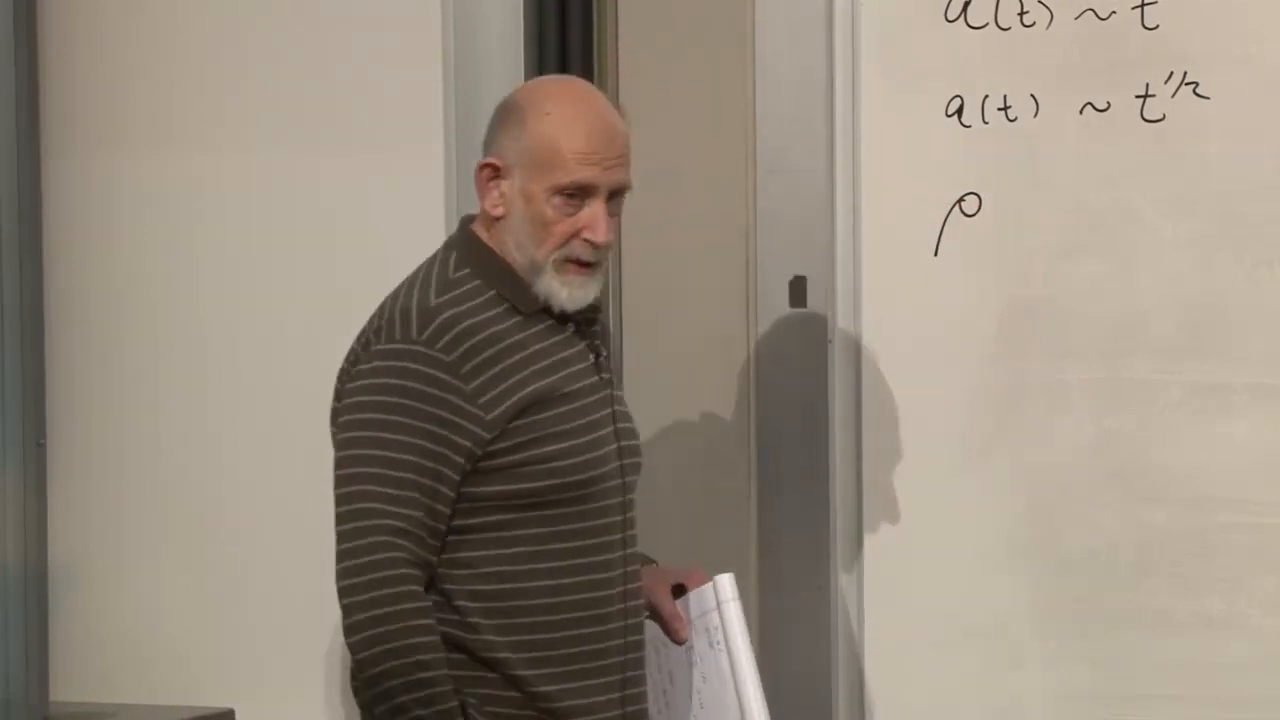
\includegraphics[width=0.72\textwidth]{lecture_05_figure_02.png}
\caption{Leyes de potencias del factor de escala repasadas y nuevo símbolo para la densidad. Es una pizarra de transición, no una deducción completa.}
\label{fig:c05-review-board}
\lectureframe{00:03:18.380}
\end{figure}

La conexión que falta es la ecuación de estado. Esta determina cómo cambia con el factor de escala la densidad de energía del lado derecho de la ecuación de Friedmann. Las dos leyes de referencia son
\begin{equation}
\rho_{\text{matter}}=\frac{\rho_0}{a^3},
\qquad
\rho_{\text{rad}}=\frac{\rho_0}{a^4}.
\label{eq:c05-benchmark-densities}
\end{equation}
La materia se diluye con el volumen, y el volumen es proporcional a \(a^3\). La radiación disminuye con una potencia adicional de \(a\). Queremos entender ambas reglas como consecuencias de la relación entre presión y densidad de energía.

\section{De la presión a la ley de escala de la densidad}

En general, una ecuación de estado puede depender de la densidad, la presión, la temperatura y otras variables. Para los componentes cosmológicos que consideramos aquí, adoptemos la forma útil con \(w\) constante:
\begin{equation}
P=w\rho,
\label{eq:c05-eos}
\end{equation}
donde \(w\) caracteriza el fluido. En la pizarra se usa una \(W\) mayúscula; aquí usamos la \(w\) minúscula convencional. Esta forma lineal abarca los casos importantes que veremos, pero es una hipótesis simplificadora, no una ley que cumplan todos los fluidos posibles.

En la materia no relativista, la densidad de energía está dominada por la energía en reposo. Si \(n\) es la densidad numérica y \(m\) la masa de las partículas, entonces, esquemáticamente,
\begin{equation}
\rho\simeq nmc^2.
\end{equation}
El factor \(c^2\) hace que incluso una masa en reposo pequeña sea una reserva enorme de energía; la aniquilación completa de un grano de polvo liberaría una cantidad macroscópica. La presión, en cambio, se produce por la transferencia de momento cuando las partículas chocan contra una pared, y es del orden de \(nmv^2\). Una bola de bolos transfiere más momento que una pelota de pimpón, pero en un gas frío toda velocidad relevante cumple \(v\ll c\). Por tanto,
\begin{equation}
\frac{P}{\rho}\sim\frac{v^2}{c^2}\ll1,
\qquad
w\simeq0.
\label{eq:c05-dust-eos}
\end{equation}
La radiación se mueve a \(c\), así que no se ajustará a esta aproximación. Deduciremos su valor de \(w\) en vez de suponerlo.

Ahora necesitamos un procedimiento general que convierta la ecuación~\eqref{eq:c05-eos} en una ley de escala para \(\rho\). Basta con una caja de laboratorio. No podemos meter literalmente las galaxias en una caja, pero, tras promediar a gran escala, se comportan como partículas, y la relación entre energía y presión puede deducirse localmente.

\begin{figure}[htbp]
\centering
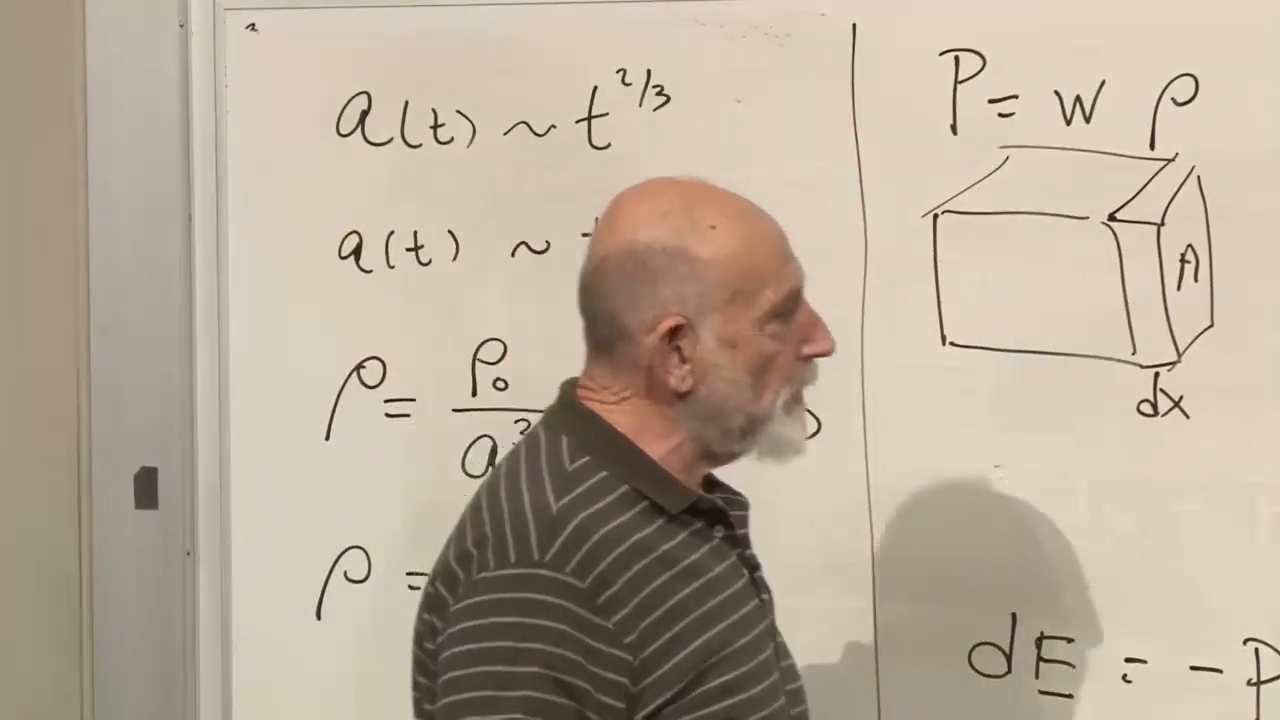
\includegraphics[width=0.86\textwidth]{lecture_05_figure_03.png}
\caption{La ecuación de estado, las escalas de densidad repasadas y la caja termodinámica en una misma pizarra. El profesor tapa parte de lo escrito anteriormente; por eso, la imagen sirve para mostrar la disposición y las ecuaciones visibles, no como transcripción completa.}
\label{fig:c05-box-board}
\lectureframe{00:13:39.612}
\end{figure}

En el lado izquierdo de la pizarra aparecen las escalas cosmológicas repasadas; en el derecho empieza el argumento de la caja. En conjunto, el contenido visible conecta
\begin{equation}
\rho_{\text{matter}}=\frac{\rho_0}{a^3},
\qquad
\rho_{\text{rad}}=\frac{\rho_0}{a^4},
\qquad
P=w\rho.
\end{equation}
Nuestro objetivo es deducir las dos leyes de densidad a partir de la ecuación de estado.

Una pared tiene área \(A\). Desplacémosla hacia fuera una distancia \(dx\), de modo que
\begin{equation}
dV=A\,dx.
\end{equation}
La presión es la fuerza por unidad de área, así que la fuerza sobre la pared es \(PA\). El gas realiza un trabajo \(PA\,dx=P\,dV\), y la energía que queda dentro disminuye.
\begin{equation}
dE=-P\,dV.
\label{eq:c05-work-law}
\end{equation}
\begin{figure}[htbp]
\centering
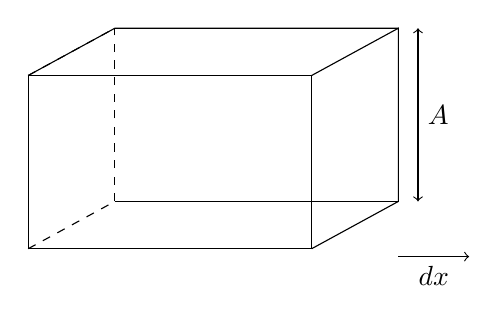
\begin{tikzpicture}[scale=1.0]
\draw (0,0) -- (3.6,0) -- (3.6,2.2) -- (0,2.2) -- cycle;
\draw (3.6,0) -- (4.7,0.6) -- (4.7,2.8) -- (3.6,2.2);
\draw (0,2.2) -- (1.1,2.8) -- (4.7,2.8);
\draw (1.1,0.6) -- (4.7,0.6);
\draw[dashed] (0,0) -- (1.1,0.6);
\draw[dashed] (0,2.2) -- (1.1,2.8);
\draw[dashed] (1.1,0.6) -- (1.1,2.8);
\draw[<->] (4.95,0.6) -- (4.95,2.8);
\node[right] at (4.95,1.7) {\(A\)};
\draw[->] (4.7,-0.1) -- (5.6,-0.1);
\node[below] at (5.15,-0.1) {\(dx\)};
\end{tikzpicture}
\caption{Reconstrucción limpia de la caja termodinámica, con área de la cara \(A\) y desplazamiento \(dx\).}
\label{fig:c05-box-redraw}
\end{figure}

La energía total es
\begin{equation}
E=\rho V.
\end{equation}
Al derivar, obtenemos
\begin{equation}
d(\rho V)=\rho\,dV+V\,d\rho.
\end{equation}
Al sustituir en la ecuación~\eqref{eq:c05-work-law}, resulta
\begin{equation}
\rho\,dV+V\,d\rho=-P\,dV.
\end{equation}
Sustituyamos \(P=w\rho\):
\begin{equation}
V\,d\rho=-(1+w)\rho\,dV.
\end{equation}
El resultado es un paso previo a la ecuación útil, pero aún no hemos llegado a ella. Dividamos entre \(\rho V\).
\begin{equation}
\frac{d\rho}{\rho}=-(1+w)\frac{dV}{V}.
\end{equation}
\begin{figure}[htbp]
\centering
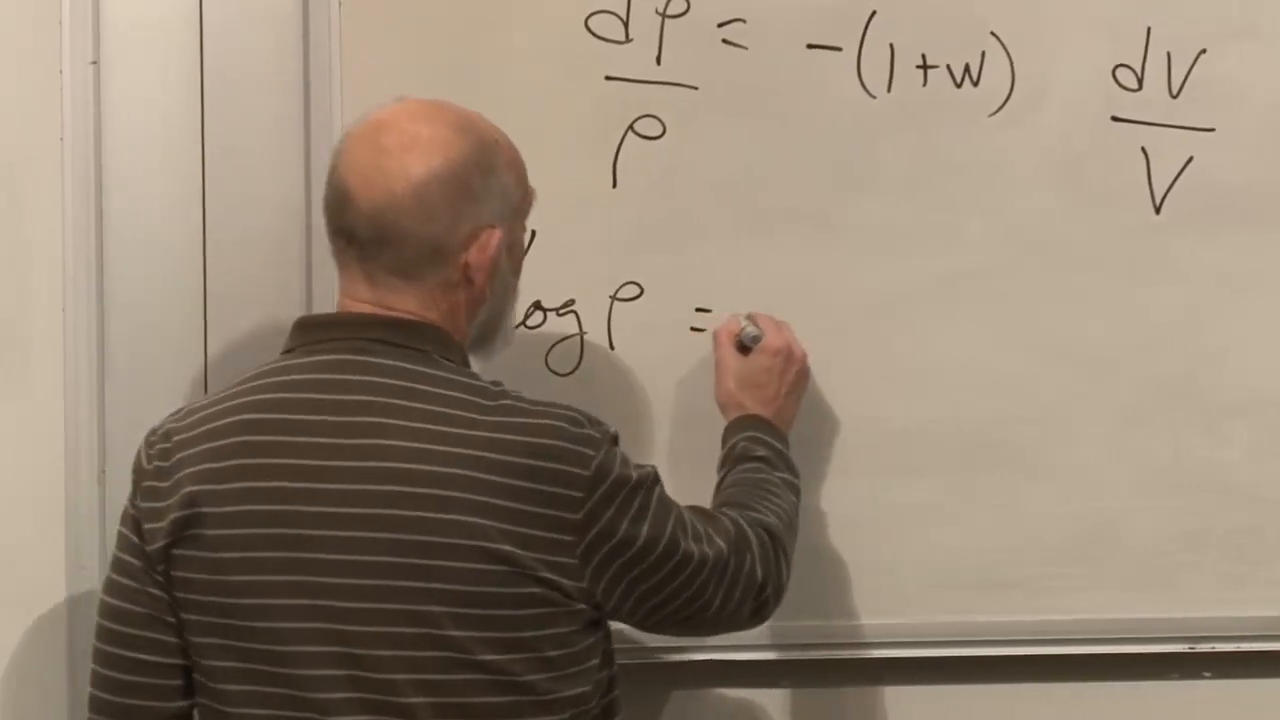
\includegraphics[width=0.78\textwidth]{lecture_05_figure_04.png}
\caption{Ecuación de densidad y volumen separada y comienzo de la integración logarítmica. El lado derecho completo se reconstruye a partir del álgebra anterior, no de los píxeles ocultos.}
\label{fig:c05-log-board}
\lectureframe{00:15:35.600}
\end{figure}

La imagen muestra la ecuación separada y el comienzo de \(\log\rho=\). Completemos la integración directamente:
\begin{equation}
d(\log\rho)=-(1+w)\,d(\log V),
\end{equation}
de modo que
\begin{equation}
\log\rho=-(1+w)\log V+\text{const.}
\end{equation}
Al exponenciar,
\begin{equation}
\rho\propto V^{-(1+w)}.
\end{equation}
Esta es la ley de densidad y volumen.

Volvamos ahora de la caja a la cosmología. Desplazar una sola pared fue una forma práctica de hacer la deducción, no una hipótesis anisotrópica. Si las tres direcciones se expanden uniformemente, se obtiene la misma relación de trabajo, y un volumen comóvil es proporcional a
\begin{equation}
V\propto a^3.
\end{equation}
Por tanto,
\begin{equation}
\boxed{\rho\propto a^{-3(1+w)}}.
\label{eq:c05-density-scaling}
\end{equation}
En \(d\) dimensiones espaciales, el exponente \(3\) pasaría a ser \(d\); el resto del argumento no cambia.

\section{Primeras aplicaciones: materia y radiación}

Ahora podemos recuperar las fórmulas repasadas como consecuencias, en vez de como hipótesis.

Para la materia no relativista, tomamos
\begin{equation}
w=0.
\end{equation}
Entonces,
\begin{equation}
\rho\propto a^{-3},
\end{equation}
que es exactamente la ley de dilución de la materia.

Para la radiación, supongamos provisionalmente que
\begin{equation}
w=\frac13.
\end{equation}
Si esto es correcto, entonces
\begin{equation}
\rho\propto a^{-3(1+1/3)}=a^{-4}.
\end{equation}
Por tanto, la potencia inversa adicional equivale a \(w=1/3\). Lo que falta es deducir ese valor a partir de la física de los fotones.

\section{Por qué la presión de radiación es un tercio de su densidad de energía}

La radiación puede describirse como ondas electromagnéticas o como partículas sin masa. Usemos fotones y calculemos la presión de un gas de fotones en una caja. La caja se dibuja en dos dimensiones, pero el gas y su distribución angular son tridimensionales. Los fotones se mueven a la velocidad de la luz y rebotan elásticamente en las paredes provisionales.

Por el momento, supongamos que todos los fotones tienen la misma energía \(\epsilon\). Esta simplificación desaparecerá al sumar las contribuciones de distintas energías. Sea \(\vec{\pi}\) el vector de momento de un fotón; evitamos usar la notación habitual \(p\) porque \(P\) ya representa la presión. Una partícula sin masa satisface las siguientes relaciones.
\begin{equation}
\epsilon=c\,\pi,
\end{equation}
con \(\pi=|\vec{\pi}|\). En las unidades empleadas en la lección, \(c=1\), así que
\begin{equation}
\epsilon=\pi.
\end{equation}
Si \(\nu\) es la densidad numérica de fotones, la densidad de energía es
\begin{equation}
\rho=\epsilon\,\nu.
\end{equation}
Tomemos el eje \(x\) perpendicular a una pared. Durante un intervalo breve \(\Delta t\), un fotón que se mueve con un ángulo \(\theta\) respecto de esa normal llega a la pared solo si parte de una lámina de grosor
\begin{equation}
\Delta x=\Delta t\cos\theta.
\end{equation}
Al reflejarse, la componente \(x\) de su momento cambia de signo, de modo que la transferencia de momento a la pared es
\begin{equation}
\Delta \pi_x=2\epsilon\cos\theta.
\end{equation}
La fuerza es la transferencia de momento por unidad de tiempo, así que cada impacto aporta \(\Delta \pi_x/\Delta t\). En la lámina hay \(\nu A\Delta x\) fotones, pero solo la mitad se mueve hacia la pared; por tanto, el número pertinente es \(\tfrac12 \nu A\Delta x\). Al dividir la fuerza total entre el área de la pared \(A\), obtenemos
\begin{align}
P(\theta)
&=
\frac{1}{A}
\left(\frac{2\epsilon\cos\theta}{\Delta t}\right)
\left(\frac12 \nu A\Delta x\right) \\
&=
\epsilon\nu\cos\theta\frac{\Delta x}{\Delta t} \\
&=
\epsilon\nu\cos^2\theta \\
&=
\rho\cos^2\theta.
\end{align}
El resultado depende del ángulo porque solo es la contribución de los fotones que viajan en una dirección.

\begin{figure}[htbp]
\centering
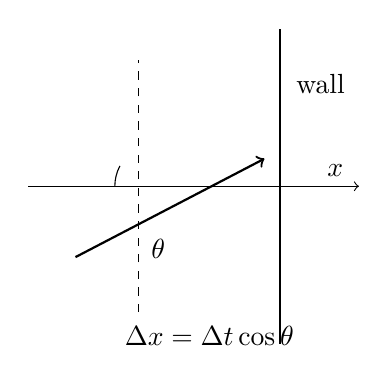
\begin{tikzpicture}[scale=1.0]
\draw[thick] (0,0) -- (0,4);
\draw[->] (-3.2,2) -- (1.0,2);
\node[above] at (0.7,2) {\(x\)};
\draw[dashed] (-1.8,0.4) -- (-1.8,3.6);
\node[below] at (-0.9,0.35) {\(\Delta x=\Delta t\cos\theta\)};
\draw[->,thick] (-2.6,1.1) -- (-0.2,2.35);
\node[below] at (-1.55,1.45) {\(\theta\)};
\draw (-2.1,2) arc[start angle=180,end angle=152,radius=0.55];
\node[right] at (0.08,3.3) {wall};
\end{tikzpicture}
\caption{Momento lineal del fotón incidente en una pared con ángulo \(\theta\), geometría utilizada para derivar la presión de radiación.}
\label{fig:c05-photon-pressure}
\end{figure}

Promediemos sobre la distribución isotrópica. Sea \(\mathbf n=(n_x,n_y,n_z)\) el vector unitario en la dirección de un fotón. Entonces,
\begin{equation}
n_x=\cos\theta,
\qquad
n_x^2+n_y^2+n_z^2=1.
\end{equation}
En un gas isotrópico, los promedios de \(n_x^2\), \(n_y^2\) y \(n_z^2\) son iguales. Al promediar la identidad anterior,
\begin{equation}
\langle n_x^2\rangle+\langle n_y^2\rangle+\langle n_z^2\rangle=1,
\end{equation}
y, por simetría, cada término es igual, así que
\begin{equation}
\langle n_x^2\rangle=\langle \cos^2\theta\rangle=\frac13.
\end{equation}
Por tanto,
\begin{equation}
P=\rho\langle \cos^2\theta\rangle=\frac{\rho}{3}.
\end{equation}
Así pues, la ecuación de estado de la radiación es
\begin{equation}
P=\frac13\rho,
\qquad
w=\frac13.
\end{equation}
El factor \(1/3\) representa el número de direcciones espaciales que comparten el cuadrado del vector unitario. En \(d\) dimensiones espaciales isotrópicas, el mismo argumento daría \(\langle n_x^2\rangle=1/d\). Con esto se completa la deducción microscópica anunciada al comienzo.

\subsection{Preguntas para comprobar el argumento sobre la radiación}

\begin{classroomqa}
\audiencequestion{¿Es necesario que todos los fotones tengan la misma energía?}
\lecturerresponse{No. Haga el cálculo por separado en cada intervalo de energía. Cada intervalo aporta una presión igual a un tercio de su propia densidad de energía, así que al sumar todo el espectro se conserva \(P=\rho/3\). Suponer que todos tenían la misma energía solo permitía abreviar la notación. \lecturetimestamp{00:39:08--00:39:36}}
\end{classroomqa}

\begin{classroomqa}
\audiencequestion{¿Se obtendría el mismo resultado con paredes negras absorbentes que con espejos perfectos, y qué papel desempeña la pared en el espacio vacío?}
\lecturerresponse{Una pared negra en equilibrio térmico absorbe y vuelve a emitir radiación, y produce el mismo balance medio de momento. El espacio cosmológico no tiene una pared literal: la superficie es una frontera imaginaria. Por cada fotón que cruza hacia fuera, la isotropía proporciona un flujo medio compensatorio hacia dentro, de modo que el cálculo local del flujo de momento no cambia. La radiación que se estudia en clase es principalmente la radiación térmica de fondo cósmico de microondas, para la cual esta imagen de equilibrio resulta especialmente natural. \lecturetimestamp{00:39:37--00:41:19}}
\end{classroomqa}

\begin{classroomqa}
\audiencequestion{¿Las estadísticas cuánticas modifican \(P=\rho/3\)?}
\lecturerresponse{No. La estadística de Bose determina cómo ocupan los fotones los modos disponibles y, por tanto, determina el espectro y \(\rho\) total; sin embargo, el esfuerzo isotrópico de las partículas sin masa sigue siendo un tercio de esa densidad de energía. \lecturetimestamp{00:41:51--00:42:02}}
\end{classroomqa}

\begin{classroomqa}
\audiencequestion{¿Qué ocurre si los fotones dispersan unos con otros?}
\lecturerresponse{La dispersión ordinaria entre fotones es extremadamente débil, así que aquí su corrección es despreciable. A temperaturas y densidades suficientemente altas, las colisiones pueden crear pares electrón-positrón y modificar el contenido efectivo de partículas y la ecuación de estado. Es un efecto real, pero corresponde a un régimen mucho más caliente que el considerado en este argumento. \lecturetimestamp{00:42:02--00:43:08}}
\end{classroomqa}

\begin{classroomqa}
\audiencequestion{¿Qué pasó con el área de la pared \(A\)?}
\lecturerresponse{El producto intermedio es la fuerza debida a un fotón multiplicada por el número de fotones que golpean la pared, y ese número es proporcional a \(A\). La presión es la fuerza dividida por el área, así que la división final cancela \(A\). La omisión en la pizarra fue llamar presión demasiado pronto a la expresión intermedia; al restablecer el paso de fuerza a presión se corrige. \lecturetimestamp{00:43:11--00:44:01}}
\end{classroomqa}

\section{Presión negativa y el significado de la tensión}

Hasta ahora, las partículas han golpeado las paredes y las han empujado hacia fuera. Esa imagen produce de forma natural una presión positiva, pero no agota las posibilidades.

\begin{classroomqa}
\audiencequestion{¿Puede ser negativa la propia densidad de energía?}
\lecturerresponse{La teoría cuántica permite densidades de energía negativas en circunstancias limitadas, y formalmente la constante cosmológica puede tener cualquiera de los dos signos. Estos casos requieren cuidado y no son el punto de partida inmediato. La posibilidad más familiar es la \emph{presión} negativa, que puede darse incluso cuando la densidad de energía es positiva. \lecturetimestamp{00:44:25--00:44:59}}
\end{classroomqa}

\begin{classroomqa}
\audiencequestion{¿Cómo puede ser negativa la presión?}
\lecturerresponse{En un mundo unidimensional, una caja es un segmento de recta. Las partículas que se mueven libremente rebotan en sus extremos y empujan hacia fuera, lo que da una presión positiva. Unamos los extremos con una cuerda o un resorte estirado. Al separarlos, el resorte tira de ellos hacia dentro. Esa fuerza hacia dentro es la tensión, el modelo unidimensional de la presión negativa. \lecturetimestamp{00:45:04--00:46:31}}
\end{classroomqa}

\begin{figure}[htbp]
\centering
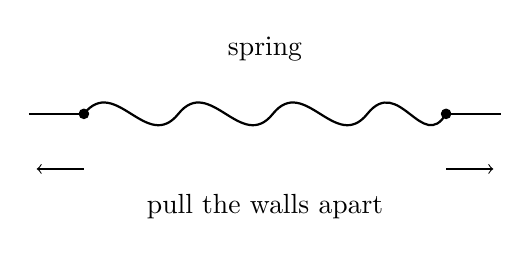
\begin{tikzpicture}[scale=1.0]
\draw[thick] (-3,0) -- (-2.3,0);
\draw[thick] (2.3,0) -- (3,0);
\draw[fill] (-2.3,0) circle (0.06);
\draw[fill] (2.3,0) circle (0.06);
\draw[thick] (-2.3,0)
.. controls (-1.9,0.5) and (-1.5,-0.5) .. (-1.1,0)
.. controls (-0.7,0.5) and (-0.3,-0.5) .. (0.1,0)
.. controls (0.5,0.5) and (0.9,-0.5) .. (1.3,0)
.. controls (1.7,0.5) and (2.0,-0.5) .. (2.3,0);
\draw[->] (-2.3,-0.7) -- (-2.9,-0.7);
\draw[->] (2.3,-0.7) -- (2.9,-0.7);
\node[below] at (0,-0.9) {pull the walls apart};
\node[above] at (0,0.55) {spring};
\end{tikzpicture}
\caption{Un resorte unidimensional como analogía de la presión negativa.}
\label{fig:c05-tension}
\end{figure}

El balance del trabajo se invierte en consecuencia. Al expandirse, un gas con presión positiva realiza trabajo y pierde energía interna. Al tirar hacia fuera contra la tensión, se almacena energía en el resorte. En términos más generales, los constituyentes atractivos pueden atraerse entre sí y tirar de la frontera hacia dentro. Así, un sistema puede tener \(\rho>0\) y \(P<0\), lo que da \(w<0\), sin contradicción alguna. Esta posibilidad es fundamental, porque la energía del vacío presenta precisamente ese patrón de signos.

\section{La energía del vacío y la constante cosmológica}

La energía del vacío se atribuye al propio espacio vacío. La teoría cuántica de campos la motiva mediante el movimiento de punto cero de los osciladores armónicos asociados a los modos de campo, pero su descripción macroscópica no exige resolver ese problema microscópico. La propiedad definitoria es que el espacio vacío tiene la misma densidad de energía cualquiera que sea el lugar o el tamaño de la región elegida.
\begin{equation}
\rho=\rho_0=\text{const.}
\label{eq:c05-vacuum-density}
\end{equation}
Si una región de volumen \(V\) contiene únicamente energía del vacío, la energía total en esa región es
\begin{equation}
E=\rho_0 V.
\end{equation}
\begin{classroomqa}
\audiencequestion{¿Una caja cambia la densidad del vacío al restringir los modos de campo permitidos?}
\lecturerresponse{La energía total en una región finita es menor que la energía en todo el espacio porque la región tiene menos volumen; la densidad a granel \(\rho_0\) permanece igual. Las fronteras reales pueden modificar las energías de los modos y producir el efecto Casimir, pero esa corrección es relevante cuando las separaciones son comparables con las longitudes de onda pertinentes. No es la densidad del vacío a gran escala que se usa en cosmología. \lecturetimestamp{00:50:06--00:51:25}}
\end{classroomqa}

Introduzcamos
\begin{equation}
\Lambda=\frac{8\pi G}{3}\rho_0.
\label{eq:c05-lambda-definition}
\end{equation}
Esta definición incorpora la combinación que aparece en la ecuación de Friedmann. La relación inversa es
\begin{equation}
\rho_0=\frac{3\Lambda}{8\pi G}.
\end{equation}
El parámetro \(\Lambda\) es la constante cosmológica. Un componente positivo y casi constante que impulsa la aceleración tardía suele llamarse energía oscura.

La dependencia con el factor de escala ya está establecida, así que invirtamos el argumento de la caja para averiguar cuál es su presión. Como \(d\rho_0=0\),
\begin{equation}
dE=d(\rho_0V)=\rho_0\,dV.
\end{equation}
Por otro lado, la relación termodinámica del trabajo sigue siendo
\begin{equation}
dE=-P\,dV.
\end{equation}
Si escribimos \(P=w\rho_0\), entonces
\begin{equation}
dE=-w\rho_0\,dV.
\end{equation}
Al comparar, resulta
\begin{equation}
w=-1.
\end{equation}
y, por tanto,
\begin{equation}
P=-\rho.
\end{equation}
La analogía del resorte anticipaba este signo. La energía positiva del vacío tiene presión negativa; la energía negativa del vacío tiene presión positiva. Las mediciones astronómicas de \(w\) permiten comprobar si el componente tardío se comporta realmente como un vacío que no se diluye: cuanto más se aproxima \(w\) a \(-1\), más se acerca el comportamiento al de la ecuación~\eqref{eq:c05-vacuum-density}.

\begin{classroomqa}
\audiencequestion{¿Es \(P=-\rho\) la ecuación de estado de un universo vacío, y podemos calcular \(\rho_0\)?}
\lecturerresponse{Es la ecuación de estado del espacio vacío cuando hay energía del vacío. Su magnitud es mucho más difícil de determinar. Todos los campos cuánticos y todas las escalas de energía pueden contribuir, incluidos campos aún no descubiertos, así que ningún cálculo aceptado explica el valor observado. El enigma principal no es cómo escribir \(w=-1\), sino por qué el \(\rho_0\) neto es extraordinariamente pequeño. \lecturetimestamp{00:57:27--00:58:29}}
\end{classroomqa}

\section{La energía del vacío en la dinámica de Friedmann}

Aislemos la energía del vacío tal como antes aislamos la materia pura y la radiación pura. Con \(\rho=\rho_0\), la ecuación de Friedmann queda
\begin{equation}
\left(\frac{\dot a}{a}\right)^2=\Lambda-\frac{k}{a^2},
\label{eq:c05-vacuum-friedmann}
\end{equation}
con \(k=+1,0,-1\) para los espacios esférico, plano e hiperbólico. Los signos positivo y negativo de \(\Lambda\), combinados con las tres opciones de \(k\), dan seis casos de signos, aunque no todos admiten soluciones reales.

\begin{remark}
En la lección se define \(\Lambda=(8\pi G/3)\rho_0\), así que aquí \(\Lambda\) tiene dimensiones de \(H^2\). En la convención habitual \(G_{\mu\nu}+\Lambda_{\mathrm E}g_{\mu\nu}=8\pi G T_{\mu\nu}\), el parámetro correspondiente es \(\Lambda_{\mathrm E}=3\Lambda\).
\end{remark}

\subsection{Expansión plana de de Sitter}

Fijemos \(k=0\). Entonces,
\begin{equation}
\left(\frac{\dot a}{a}\right)^2=\Lambda.
\end{equation}
Para \(\Lambda>0\), elijamos la rama expansiva:
\begin{equation}
\dot a=\sqrt{\Lambda}\,a,
\end{equation}
y, por tanto,
\begin{equation}
a(t)=C\,e^{\sqrt{\Lambda}\,t}.
\end{equation}
El parámetro de Hubble es entonces constante:
\begin{equation}
H=\frac{\dot a}{a}=\sqrt{\Lambda}.
\end{equation}
Este es el espacio de de Sitter en foliación plana, llamado así por Willem de Sitter, quien obtuvo la solución con constante cosmológica poco después de que Einstein introdujera ese término en 1917. Si \(\Lambda<0\) mientras que \(k=0\), la ecuación~\eqref{eq:c05-vacuum-friedmann} no tiene soluciones reales porque \(H^2\) no puede ser negativo.

\begin{classroomqa}
\audiencequestion{¿Es realmente constante aquí el parámetro de Hubble, y tiene este espacio-tiempo un big bang?}
\lecturerresponse{Para la solución pura en foliación plana, \(H=\sqrt{\Lambda}\) es exactamente constante. Aunque \(a(t)\to0\) solo cuando \(t\to-\infty\), esta carta coordenada no es geodésicamente completa: algunas trayectorias dirigidas hacia el pasado llegan a su frontera en un tiempo propio finito. Por tanto, la fórmula por sí sola no resuelve la cuestión del big bang global. La geometría completa de de Sitter contiene más que esta carta plana; este asunto se pospone hasta estudiar la geometría en detalle. \lecturetimestamp{01:06:54--01:08:07}}
\end{classroomqa}

Una ecuación esquemática de Friedmann para un universo con materia, radiación, curvatura y energía del vacío es
\begin{equation}
\left(\frac{\dot a}{a}\right)^2
=
\Lambda+\frac{C_m}{a^3}+\frac{C_r}{a^4}-\frac{k}{a^2}.
\label{eq:c05-mixed-friedmann}
\end{equation}
En los primeros tiempos, cuando \(a\) es pequeño, dominan las potencias inversas y la energía del vacío es despreciable. En los tiempos tardíos, cuando \(a\) es grande, domina el término constante \(\Lambda\). Así pues, el universo atraviesa una transición: al principio parece dominado por la materia o la radiación, mientras que al final se aproxima a un comportamiento de tipo de Sitter.

Una exponencial tiene \(\ddot a>0\), así que la dominación del vacío implica expansión acelerada. Durante la transición, la aceleración no tiene por qué ser exactamente exponencial, porque la materia todavía contribuye a la ecuación~\eqref{eq:c05-mixed-friedmann}. Se describe que las observaciones de la época de la lección captan al universo durante esta competencia, no en una fase de de Sitter pura ya establecida.

\section{Preguntas sobre la energía del vacío}

\begin{classroomqa}
\audiencequestion{Si la energía del vacío es energía del estado fundamental, ¿cómo puede ser negativa?}
\lecturerresponse{Un modo de oscilador bosónico aporta \(+\tfrac12\hbar\omega\), mientras que un modo fermiónico aporta una contribución con el signo opuesto. La energía neta del vacío es una suma sobre muchos campos y escalas, así que puede tener cualquiera de los dos signos antes de conocer el total. La existencia de contribuciones es natural; lo difícil es explicar el residuo extraordinariamente pequeño. \lecturetimestamp{01:12:00--01:14:12}}
\end{classroomqa}

\begin{classroomqa}
\audiencequestion{¿Una \(w=-1\) constante implica un big rip futuro?}
\lecturerresponse{No. Una constante cosmológica con \(w=-1\) da lugar a una expansión exponencial de tipo de Sitter, pero no produce la divergencia en tiempo finito llamada big rip. Ese escenario corresponde a un componente fantasma hipotético con \(w<-1\), para el cual la densidad crece a medida que el universo se expande. Aquí no se supone que exista tal componente. \lecturetimestamp{01:14:13--01:15:50}}
\end{classroomqa}

\begin{classroomqa}
\audiencequestion{¿La supersimetría exacta haría desaparecer la energía del vacío?}
\lecturerresponse{Puede cancelar las contribuciones de punto cero porque cada grado de libertad bosónico tiene como pareja uno fermiónico. Sin embargo, la naturaleza no presenta supersimetría exacta a bajas energías: los bosones y fermiones observados no tienen parejas con la misma masa. Por tanto, la cancelación exacta no explica la energía del vacío en el mundo tal como lo observamos actualmente. \lecturetimestamp{01:15:51--01:16:20}}
\end{classroomqa}

\begin{classroomqa}
\audiencequestion{¿Cuál es la enorme discrepancia entre una estimación natural de la energía del vacío y el valor observado?}
\lecturerresponse{Las constantes universales \(c\), \(\hbar\) y \(G\) definen las unidades de Planck. La velocidad \(c\) limita todas las señales, \(\hbar\) fija la escala universal de incertidumbre cuántica y \(G\) acopla toda energía a la gravedad. Con ellas se construye una masa de Planck del orden de \(10^{-5}\) gramos y una longitud de Planck del orden de \(10^{-33}\) centímetros; de ahí se obtiene una densidad de energía de Planck de aproximadamente una energía de Planck por longitud de Planck cúbica. En esas unidades, en la lección se cifra la densidad observada del vacío en torno a \(10^{-123}\), aunque el exponente exacto depende de la convención. El misterio es por qué unas contribuciones que sugieren de manera natural una escala mucho mayor dejan un resultado no nulo tan pequeño. \lecturetimestamp{01:16:21--01:23:12}}
\end{classroomqa}

\begin{classroomqa}
\audiencequestion{¿Por qué sorprendió a los físicos descubrir una constante cosmológica distinta de cero si se esperan contribuciones del vacío?}
\lecturerresponse{Las sucesivas mejoras observacionales seguían arrojando un resultado compatible con cero. Esa historia alimentó la expectativa psicológica de que algún principio exacto desconocido, quizá una futura teoría de la gravedad cuántica, imponía la cancelación completa. El descubrimiento posterior desbarató esa expectativa. La sorpresa reflejaba décadas de resultados nulos cada vez más precisos, no una deducción de que la energía del vacío debía anularse. \lecturetimestamp{01:23:14--01:26:05}}
\end{classroomqa}

\begin{classroomqa}
\audiencequestion{¿Pueden las observaciones determinar si la energía oscura cambia con el tiempo?}
\lecturerresponse{No pueden descartar un cambio brusco en un futuro remoto, pero sí comparar la historia reciente de expansión a lo largo de miles de millones de años. Medir \(w\) o, en general, \(w(a)\) permite comprobar si la densidad ha evolucionado durante ese intervalo. En la lección se informa de que la restricción vigente entonces solo tenía una precisión aproximada del diez por ciento; esa cifra es histórica, mientras que el punto perdurable es que \(w=-1\) corresponde a una densidad invariable. \lecturetimestamp{01:26:06--01:27:16}}
\end{classroomqa}

\begin{classroomqa}
\audiencequestion{¿Cambiaría el resultado con otro número de dimensiones espaciales?}
\lecturerresponse{La estructura general se mantiene. En \(d\) dimensiones espaciales isotrópicas, la radiación tiene \(w=1/d\) y se diluye como \(a^{-(d+1)}\), mientras que la energía del vacío invariante de Lorentz sigue teniendo \(w=-1\). Los coeficientes numéricos de la ecuación de Friedmann cambian con la dimensión, pero se conserva la distinción entre materia y radiación que se diluyen y un vacío que no se diluye. \lecturetimestamp{01:27:16--01:27:57}}
\end{classroomqa}

\section{Curvatura y analogía mecánica}

\subsection{Curvatura positiva con energía positiva del vacío}

Tomemos \(k=+1\) y \(\Lambda>0\):
\begin{equation}
\left(\frac{\dot a}{a}\right)^2=\Lambda-\frac{1}{a^2}.
\label{eq:c05-closed-vacuum}
\end{equation}
Multiplicando por \(a^2\),
\begin{equation}
\dot a^2-\Lambda a^2=-1.
\label{eq:c05-inverted-oscillator}
\end{equation}
Interpretemos \(a\) como la coordenada de una partícula ficticia. Entonces \(\dot a^2\) es su término cinético, \(-\Lambda a^2\) es un potencial cuadrático invertido y la energía total es \(-1\). La rama físicamente permitida cumple \(a\geq\Lambda^{-1/2}\): el universo se contrae desde un tamaño grande, se detiene al llegar al mínimo y vuelve a expandirse.

La solución exacta es
\begin{equation}
a(t)=\Lambda^{-1/2}\cosh(\sqrt{\Lambda}\,t).
\label{eq:c05-closed-desitter}
\end{equation}
Usando
\begin{equation}
\cosh(\sqrt{\Lambda}\,t)
=
\frac12\left(e^{\sqrt{\Lambda}\,t}+e^{-\sqrt{\Lambda}\,t}\right),
\end{equation}
La función es simétrica en el tiempo. En \(t=0\), \(a=\Lambda^{-1/2}\); al avanzar en cualquiera de los dos sentidos temporales, crece exponencialmente. Por tanto, la foliación cerrada muestra una contracción, un mínimo no singular y una nueva expansión. Su aspecto global difiere del de la foliación exponencial plana, pero ambos sistemas de coordenadas cubren partes de la misma geometría de de Sitter.

\subsection{Constante cosmológica negativa}

Escribamos \(\Lambda=-|\Lambda|\). Si \(k=+1\), la ecuación~\eqref{eq:c05-vacuum-friedmann} tiene un lado derecho negativo para todo \(a\), mientras que \(H^2\geq0\). No existe ninguna solución FRW real de este tipo con vacío puro.

Para \(k=-1\),
\begin{equation}
\left(\frac{\dot a}{a}\right)^2=-|\Lambda|+\frac{1}{a^2}.
\end{equation}
Multiplicando ambos lados por \(a^2\),
\begin{equation}
\dot a^2+|\Lambda|a^2=1.
\label{eq:c05-negative-lambda-oscillator}
\end{equation}
Esta es la ecuación de energía de un oscilador armónico. Como \(a\geq0\), un semiperiodo físico es
\begin{equation}
a(t)=\frac{1}{\sqrt{|\Lambda|}}
\sin\!\left(\sqrt{|\Lambda|}\,t\right),
\qquad
0<t<\frac{\pi}{\sqrt{|\Lambda|}}.
\end{equation}
El universo abierto comienza en \(a=0\), alcanza \(a_{\max}=|\Lambda|^{-1/2}\) y vuelve a un big crunch. Por tanto, una geometría espacial abierta no garantiza una expansión eterna: una constante cosmológica negativa puede invertirla. Un valor muy grande y positivo de \(\Lambda\) desgarraría las estructuras ligadas, mientras que un valor muy grande y negativo provocaría una recolisión rápida.

\begin{figure}[htbp]
\centering
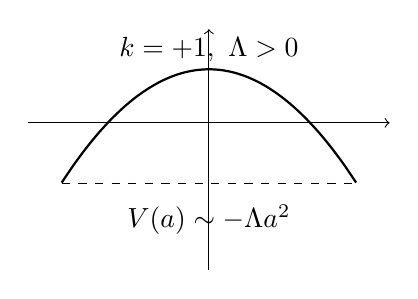
\begin{tikzpicture}[scale=0.85]
\draw[->] (-2.7,0) -- (2.7,0);
\draw[->] (0,-2.2) -- (0,1.4);
\draw[thick,domain=-2.2:2.2,smooth] plot (\x,{-0.35*(\x)^2 + 0.8});
\draw[dashed] (-2.2,-0.9) -- (2.2,-0.9);
\node at (0,-1.45) {\(V(a)\sim -\Lambda a^2\)};
\node at (0,1.1) {\(k=+1,\ \Lambda>0\)};
\end{tikzpicture}
\hspace{2em}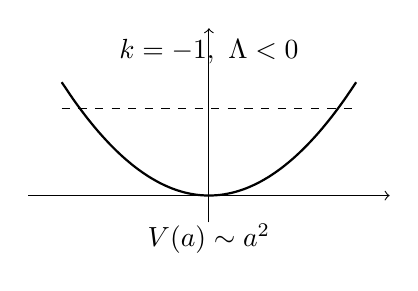
\begin{tikzpicture}[scale=0.85]
\draw[->] (-2.7,0) -- (2.7,0);
\draw[->] (0,-0.4) -- (0,2.5);
\draw[thick,domain=-2.2:2.2,smooth] plot (\x,{0.35*(\x)^2});
\draw[dashed] (-2.2,1.3) -- (2.2,1.3);
\node at (0,-0.65) {\(V(a)\sim a^2\)};
\node at (0,2.15) {\(k=-1,\ \Lambda<0\)};
\end{tikzpicture}\caption{Potenciales efectivos esquemáticos para el rebote de Sitter cerrado y el recolapso del modelo abierto con constante cosmológica \(\Lambda\) negativa.}
\label{fig:c05-mechanical-potentials}
\end{figure}

\begin{classroomqa}
\audiencequestion{¿Son estas ecuaciones de Friedmann realmente las ecuaciones de Einstein?}
\lecturerresponse{Sí. Son las ecuaciones de campo de Einstein una vez que la homogeneidad y la isotropía reducen la métrica a una sola función, \(a(t)\). La reducción por simetría elimina la mayoría de las componentes tensoriales y deja esta ecuación diferencial ordinaria para la expansión cósmica. \lecturetimestamp{01:43:52--01:44:05}}
\end{classroomqa}

\begin{classroomqa}
\audiencequestion{¿Podría ser complejo el factor de escala \(a\)?}
\lecturerresponse{No en las cosmologías FRW clásicas reales que se analizan aquí. El factor de escala mide el tamaño espacial y se considera real y no negativo. Las geometrías complejificadas pueden aparecer en otros enfoques matemáticos, pero no intervienen en las soluciones de esta clase. \lecturetimestamp{01:44:06--01:44:21}}
\end{classroomqa}

\begin{classroomqa}
\audiencequestion{¿Hay alguna razón física por la que la presión deba ser una función lineal de la densidad?}
\lecturerresponse{No. Un valor constante de \(w\) es conveniente y, además, describe los componentes principales que se consideran aquí. Una mezcla de materia, radiación y vacío no tiene un único valor constante de \(w\) en todas las épocas, y un material general puede tener una relación \(P(\rho)\) no lineal. En un fluido barótropo, \(dP/d\rho\) determina el cuadrado de la velocidad del sonido en unidades donde \(c=1\); un valor constante de \(w\) hace constante esa derivada, pero la naturaleza no está obligada a ello. \lecturetimestamp{01:44:21--01:45:34}}
\end{classroomqa}

\section{Qué conviene recordar}

La ecuación de estado conecta la física microscópica con la evolución temporal del factor de escala. El trabajo adiabático en una caja comóvil da
\[
\rho\propto a^{-3(1+w)}.
\]
La materia fría tiene \(w=0\) y \(\rho\propto a^{-3}\). El flujo isotrópico del momento de los fotones da
\[
\left\langle\cos^2\theta\right\rangle=\frac13,
\qquad
P_{\mathrm r}=\frac{\rho_{\mathrm r}}{3},
\qquad
\rho_{\mathrm r}\propto a^{-4}.
\]

La tensión hace físicamente comprensible la presión negativa. Una densidad de vacío constante cumple
\[
P_\Lambda=-\rho_\Lambda,
\qquad
w_\Lambda=-1.
\]
Una energía del vacío positiva produce una expansión exponencial de de Sitter en la foliación plana y un rebote \(\cosh\) en la foliación cerrada. Una energía del vacío negativa puede hacer que incluso un universo abierto vuelva a contraerse. Cualquiera que sea el signo, la ecuación de Friedmann puede interpretarse como una ecuación de energía mecánica efectiva. La pregunta sin resolver no es por qué los campos cuánticos contribuyen a la energía del vacío, sino por qué su contribución neta observada es casi nula, aunque no exactamente nula.
